%   % !TEX root = ../../VIII,3_Rahmen-TeX_9-0.tex
%  
%   Signatur/Tex-Datei:	LH_37_05_144-145
%   RK-Nr. 	57267_3		
%
%
%   edlabels:			29	+1 (Referenz)		
%   Diagramme: 		5
%
%
%
\selectlanguage{ngerman}
\frenchspacing
%
\begin{ledgroupsized}[r]{120mm}
\footnotesize
\pstart
\noindent\textbf{Überlieferung:}
\pend
\end{ledgroupsized}
%
\begin{ledgroupsized}[r]{114mm}
\footnotesize
\pstart \parindent -6mm
\makebox[6mm][l]{\textit{L}}%
Auszüge mit Bemerkungen aus
\protect\index{Namensregister}{\textso{Mariotte}, Edme, Seigneur de Chazeuil ca. 1620\textendash1684}%
\textsc{E.~Mariotte}, %
\cite{00311}\title{Traité de la percussion ou du chocq des corps}, %
Paris 1673:
LH~XXXVII~5~Bl.~144\textendash145. %ggf. (unsere Druckvorlage).
Ein Bogen~2\textsuperscript{o};
Wasserzeichen in der Mitte von Bl.~145;
Papiererhaltungsmaßnahmen;
Papierbruch an den Blatträndern mit Textverlust.
Zwei Drittel Seite auf Bl.~145~r\textsuperscript{o} sowie eine Zeile am oberen Rand von 145~v\textsuperscript{o}.
Bl.~144~r\textsuperscript{o} überliefert N.~\ref{57267_1}.
Bl.~144~v\textsuperscript{o} und das obere Drittel von Bl.~145~r\textsuperscript{o} überliefern N.~\ref{57267_2}.
Bl.~145~v\textsuperscript{o} und der untere linke Bereich von Bl.~144~r\textsuperscript{o} überliefern N.~\ref{57268}.
\pend
\end{ledgroupsized}
%
\begin{ledgroupsized}[r]{114mm}
\footnotesize
\count\Bfootins=1100%
\count\Afootins=1100%
\count\Cfootins=1100
\pstart
\parindent -6mm
\makebox[6mm][l]{\textit{E}}%
\textsc{Fichant} 1994, S.~361\textendash364\cite{01056}.
\pend%
\end{ledgroupsized}
%
%
\selectlanguage{latin}
\frenchspacing
% \newpage%
\vspace{8mm}
%
\pstart%
\normalsize%
\noindent%
\hspace{1mm}\hspace{-1mm}% Trick, weil \edlabel nicht zu \par-Beginn sein darf
\edlabel{37_05_144-145_23a}%Anfang der Besprechung von Mariotte
\edlabel{LH_37_05_145r_prop.I.3_Mario-1}%Referenzierung für PR
\lbrack145~r\textsuperscript{o}\rbrack\ Dubium videtur
%
\edtext{secundum principium experientiae\protect\index{Sachverzeichnis}{principium experientiae} a Mariotto%
\protect\index{Namensregister}{\textso{Mariotte}, Edme, Seigneur de Chazeuil ca. 1620\textendash1684} %
positum (second principe d'experience)%
\protect\index{Sachverzeichnis}{principe d'experience}}{%
\lemma{secundum \lbrack...\rbrack\ d'experience\protect\vphantom()}%
\Cfootnote{%
\protect\index{Namensregister}{\textso{Mariotte}, Edme, Seigneur de Chazeuil ca. 1620\textendash1684}%
\textsc{E.~Mariotte}, %
\cite{00311}\title{Traité de la percussion}, %de la percussion ou du Chocq des corps}, %
Paris 1673, %
Première partie, Prop.~III (Second principe d'experience),
S.~25\textendash29. 
Siehe auch Leibnizens Auszüge von 1674 aus 
\protect\index{Namensregister}{\textso{Mariotte}, Edme, Seigneur de Chazeuil ca. 1620\textendash1684}Mariottes
Werk (\textit{LSB} VIII, 2 N.~50\cite{01292}).%
}}
% 
% == 19 ==
%
quod ictus\protect\index{Sachverzeichnis}{ictus} corporum concurrentium sit idem\lbrack,\rbrack\ modo sit eadem 
%
celeritas appropinquationis\protect\index{Sachverzeichnis}{appropinquatio}\protect\index{Sachverzeichnis}{celeritas appropinquationis} nulla ratione habita propriarum 
% 
% == 20 ==
%
celeritatum.\protect\index{Sachverzeichnis}{celeritas propria}%
\edlabel{37_05_144-145_second_principe}	%zwecks Referenzierung
%
%
\edtext{Ita ut}{%
\lemma{}%
\Bfootnote{%
Ita \textbar\ ut \textit{streicht Hrsg.}~\textbar\ %
 ut %
\textit{L}}}
%
\pend
%
\vspace{1.0em} %%%%%%%%% Diagramm  1
\centerline{%
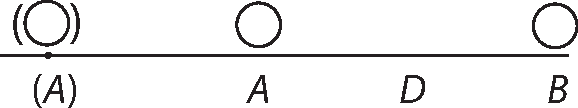
\includegraphics[width=0.42\textwidth]{%
gesamttex/edit_VIII,3/images/LH_37_05_144-145_d3_145r.pdf%
}} 
\vspace{0.5em}
\centerline{%
\lbrack\textit{Fig.~1}\rbrack%
}
% \newpage%
\vspace{0.5em}
%
\pstart\noindent
%
\edtext{\lbrack\textit{A} et \textit{B}\rbrack}{%
\lemma{}%
\Bfootnote{%
\textit{AD} et \textit{BD} %
\textit{L ändert Hrsg.}%
}}
concurrentes in \textit{D} celeritate appropinquationis,%
\protect\index{Sachverzeichnis}{celeritas appropinquationis} quae sit 
$AD + BD$\lbrack,\rbrack\
%
% == 21 ==
%
eundem sibi infligunt 
%
\edtext{ictum,\protect\index{Sachverzeichnis}{ictus} quem}{\lemma{ictum,}\Bfootnote{\textit{(1)}~quam \textit{(2)}~quem~\textit{L}}}
%
infligerent si \textit{B} quiescat  
%
\edtext{e\lbrack t\rbrack}{%
\lemma{}%
\Bfootnote{%
ex %
\textit{L ändert Hrsg.}%
}}
%
(\textit{A}) ipsi incurrat celeritate \textit{AB}, seu \textit{2AD},
%
% ==22 ==
%
seu $AD+BD$. 
%
\edtext{Sane priori}{\lemma{Sane}\Bfootnote{\textit{(1)}~si corpus \textit{(2)}~priori~\textit{L}}}
%
casu, ubi \textit{A} et \textit{B} concurrunt aequivelociter in \textit{D} vel etiam celeritate reciproca ponderibus\lbrack,\rbrack\
%
% == 23 ==
%
ictus vis%
\protect\index{Sachverzeichnis}{vis ictus} est eadem cum tota vi\protect\index{Sachverzeichnis}{vis tota} utriusque 
%
\edtext{corporis. At}{\lemma{corporis.}\Bfootnote{\textit{(1)}~Si vero \textit{(2)}~At~\textit{L}}}
% 
posteriore \edtext{casu ictus vis\protect\index{Sachverzeichnis}{vis ictus} non}{%
\lemma{}%
\Bfootnote{%
casu ictus vis \textbar\ est \textit{streicht Hrsg.}~\textbar\ %
 non~\textit{L}}}
%
est eadem 
%
cum vi
%
% == 24 ==
%
corporum, id est hoc loco solius (\textit{A}) quia si ictus\protect\index{Sachverzeichnis}{ictus} totam vim\protect\index{Sachverzeichnis}{vis tota} corporum reciperet, solus etiam ageret, ideo idem fieret 
%
% == 25 ==
%
in casu priore et posteriore, quod tamen non fit: nam praeter vim ictus\protect\index{Sachverzeichnis}{vis ictus} etiam corpus \edtext{\textit{B}}{%
\lemma{}%
\Bfootnote{%
\textit{B} %
\textit{erg.\ L}%
}}
 propellitur, non vero corpus 
%
% == 26 ==
%
(\textit{A}) vel \textit{A} ut ante repellitur. Non videtur ergo ictus\protect\index{Sachverzeichnis}{ictus} totam vim\protect\index{Sachverzeichnis}{vis tota} 
%
\makebox[1.0\textwidth][s]{\edtext{recipere ergo cum}{\lemma{recipere ergo}\Bfootnote{\textit{(1)}~non \textit{(2)}~cum~\textit{L}}}
%
%
vis\protect\index{Sachverzeichnis}{vis} corporum sit
% 
% == 27 ==
%
utrobique eadem, non erit idem ictus\protect\index{Sachverzeichnis}{ictus}  priore et poste-} 
\pend
\newpage
\pstart
\noindent riore casu, contra Hypothesin\protect\index{Sachverzeichnis}{hypothesis Mariotti} 
%
Mariotti\protect\index{Namensregister}{\textso{Mariotte}, Edme, Seigneur de Chazeuil ca. 1620\textendash1684}.%
\edlabel{LH_37_05_145r_prop.I.3_Mario-2} %Referenzierung für PR
%
\edtext{Experientiam\protect\index{Sachverzeichnis}{experientia} allegat Mariottus%
\protect\index{Namensregister}{\textso{Mariotte}, Edme, Seigneur de Chazeuil ca. 1620\textendash1684}, %
quod corpora mollia%
\protect\index{Sachverzeichnis}{corpus molle} eodem modo eadem appropinquationis quantitate%
\protect\index{Sachverzeichnis}{quantitas appropinquationis} %
comprimuntur seu complanantur (sont applatis).}{%
\lemma{Experientiam \lbrack...\rbrack\ applatis\protect\vphantom()}%
\Cfootnote{%
\protect\index{Namensregister}{\textso{Mariotte}, Edme, Seigneur de Chazeuil ca. 1620\textendash1684}%
\textsc{Mariotte}, %
\cite{00311}\title{Traité de la percussion}, % de la percussion ou du Chocq des corps}, %
Première partie, Prop.~XI (Septième principe d'experience), S.~28.%
}}
%
Videndum etiam an eundem uterque ictus\protect\index{Sachverzeichnis}{ictus} producat 
sonum.\protect\index{Sachverzeichnis}{sonus}
%
% == 30 ==
%
In Elateriis\protect\index{Sachverzeichnis}{elaterium} experientia\protect\index{Sachverzeichnis}{experientia} dabit an eodem modo utroque casu comprimantur.
%
Adhibeatur \edtext{oscillatorium spirale Elasticum\protect\index{Sachverzeichnis}{oscillatorium spirale elasticum} Hugenii\protect\index{Namensregister}{\textso{Huygens} (Hugenius, Ugenius, Hugens, Huguens), Christiaan 1629\textendash1695}.}{%
\lemma{oscillatorium \lbrack...\rbrack\ Hugenii}%
\Cfootnote{%
\protect\index{Namensregister}{\textso{Huygens} (Hugenius, Ugenius, Hugens, Huguens), Christiaan 1629\textendash1695}\textsc{C.~Huygens}, \cite{02019}\glqq Une nouvelle invention d'horloges très-justes et portatives\grqq, \cite{00157}\textit{JS} (Pariser Ausgabe), 25.~Februar 1675, S.~68\textendash70 (\cite{00113}\textit{HO} VII, S.~424f.). %
Zu Leibnizens Reaktion vgl.\ \cite{01208}\glqq Le principe de justesse des horologes portatives de son invention\grqq, \cite{00157}\textit{JS} (Pariser Ausgabe), 25. März 1675, S.~93\textendash96 (\textit{LSB} III, 1 N.~45\textsubscript{3}).%
}}
\pend \pstart
\edtext{Expertus est Mariottus\protect\index{Namensregister}{\textso{Mariotte}, Edme, Seigneur de Chazeuil ca. 1620\textendash1684} corpora mollia%
\protect\index{Sachverzeichnis}{corpus molle} concurrentia servare eandem motus  
%
\edtext{quantitatem,\protect\index{Sachverzeichnis}{quantitas motus} si celerius assequatur tarde}{\lemma{quantitatem, si}\Bfootnote{\textit{(1)}~unum \textit{(2)}~celerius assequatur \textit{(a)}~tardius \textit{(b)}~tarde~\textit{L}}}
%
praecedens seu quiescens.}{%
\lemma{Expertus \lbrack...\rbrack\ quiescens}%
\Cfootnote{%
\protect\index{Namensregister}{\textso{Mariotte}, Edme, Seigneur de Chazeuil ca. 1620\textendash1684}%
\textsc{Mariotte}, %
\cite{00311}\title{Traité de la percussion}, % de la percussion ou du Chocq des corps}, %
Première partie, Prop.~XI (Septième principe d'experience),
S.~56\textendash60, bes.\ S.~56f.%
}}
%
\edtext{Sed si sibi occurrant, tantum servatur differentia quantitatum motus\protect\index{Sachverzeichnis}{quantitas motus} quae divisa per quantitatem corporum%
\protect\index{Sachverzeichnis}{quantitas corporis} dat celeritatem totius, quemadmodum scilicet simul
procedunt.}{%
\lemma{Sed \lbrack...\rbrack\ procedunt}%
\Cfootnote{%
\cite{00311}a.a.O., %
Prop.~XII (Huitième principe d'experience),
S.~60\textendash68, bes.\ S.~60f.%
}}
 Videndum est
%
\edtext{an posita}{\lemma{an}\Bfootnote{\textit{(1)}~utroque casu \textit{(2)}~eodem modo corpora mollia \textit{(3)}~posita~\textit{L}}}
%
eadem motus 
%
\edtext{quantitate\protect\index{Sachverzeichnis}{quantitas motus} tam}{\lemma{quantitate}\Bfootnote{\textit{(1)}~vel ae \textit{(2)}~aliquando \textit{(3)}~tam~\textit{L}}}
%
in assecutione%
\protect\index{Sachverzeichnis}{assecutio} quam in occursu,%
\protect\index{Sachverzeichnis}{occursus} eorundem corporum, aliquo casu effici possit
%
% == 36 ==
%
ut eodem modo complanentur ictu\protect\index{Sachverzeichnis}{ictus} corpora, tunc enim dici non posset quod ego dico\lbrack,\rbrack\ motum perditum
%
% == 37 ==
%
recipi in materia molli.%
\protect\index{Sachverzeichnis}{materia mollis}%
\edtext{}{%
\lemma{\hspace*{1,6mm}%
\lbrack\textit{Fig.~2}\rbrack%
}\killnumber%
\Cfootnote{%
tlw.\ Übernahme der Vorlage: a.a.O, Fig.~7.%
}}% 
\pend
%
\vspace{2.0em} %%%%%%%%% Diagramm 2
\centerline{%

\includegraphics[width=0.32\textwidth]{%
gesamttex/edit_VIII,3/images/LH_37_05_144-145_d4_145r.pdf%
}} 
\vspace{0.5em}
\centerline{%
\lbrack\textit{Fig.~2}\rbrack%
}
% \newpage%
%\vspace{1.5em}
%
\newpage
\pstart
%
\edtext{}{% C-Footnote – "Regula generalis Mariotti" um eine A-Fn herum
{\xxref%
{37_05_144-145_15a}{37_05_144-145_15b}}%
\lemma{Regula \lbrack...\rbrack\  carentibus}\Cfootnote{%
\cite{00311}a.a.O., %
Prop.~XIII, S.~68\textendash72.}}
\edlabel{37_05_144-145_15a}%
\edtext{Regula generalis Mariotti%
\protect\index{Sachverzeichnis}{regula generalis Mariotti}%
\protect\index{Namensregister}{\textso{Mariotte}, Edme, Seigneur de Chazeuil ca. 1620\textendash1684}}{%
\lemma{}\Afootnote{%
\textit{Oberhalb der Zeile, mit Verweislinie auf} Mariotti:\enskip %
Ingeniose sic demonstrat:\textsuperscript{\lbrack a\rbrack} si esset celeritas et directio \textit{AC} et \textit{BC} quiescerent post concursum.\protect\index{Sachverzeichnis}{concursus} Nunc vero in \textit{A} est $AC+CD$ et in \textit{B} est $AC-CD$. Ergo illi\textsuperscript{\lbrack b\rbrack} \textit{A} additur, illi \textit{B} opposite detrahitur, id est etiam additur. Ergo post quietem utrumque eam retinet \textit{CD}, inde a \textit{D} directione \textit{CD} id est \textit{DE}.
\newline\vspace{-0.5em}\newline%Marginalienapparat:
{\footnotesize \textsuperscript{\lbrack a\rbrack} demonstrat:\ \cite{00311}a.a.O, Prop.~XIII, S.~68f.\quad %
\textsuperscript{\lbrack b\rbrack} illi \textit{(1)}~additur \textit{(2)}~\textit{A} additur, illi \textit{B} \textit{(a)}~oppositum ejus \textit{(b)}~opposite~\textit{L}\newline}}}
%
pro Corporibus Elaterio\protect\index{Sachverzeichnis}{elaterium} carentibus:%
\protect\index{Sachverzeichnis}{corpus elaterio carens}\edlabel{37_05_144-145_15b}
%
ait enim
% 
\edtext{prop.~13\lbrack:\rbrack\ \edlabel{37_05_144-145_16a}\textit{si}}{\lemma{prop.~13}\Bfootnote{\textit{(1)}~si linea \textit{AB} \textit{(2)}~\textit{si}~\textit{L}}}%
\edtext{}{% C-Footnote – "si une ligne" überkreuzt sich mit B-Fn.
{\xxref%
{37_05_144-145_16a}{37_05_144-145_16b}}%
\lemma{\textit{si} \lbrack...\rbrack\ \textit{ressort}}%
\Cfootnote{%
\cite{00311}a.a.O., S.~68 mit Auslassung.%
}}
%
\textit{une ligne comme \textit{AB} est divisée au 
point \textit{C} en raison reciproque des poids des corps \textit{A}, \textit{B}, et 
qui estant prolongée directement de part et d'autre}\lbrack,\rbrack\ 
\textit{on y prenne
un point \textit{D} en sorte qu'\textit{AD} represente 
%
\edtext{la vitesse et la direction}{\lemma{la vitesse}\Bfootnote{\textit{(1)}~du corps \textit{(2)}~\textit{et la direction}~\textit{L}}}
%
du corps \textit{A} avant le choc, et \textit{BD} celle du corps \textit{B}, l'une et l'autre
vitesse supposée} 
%
\edtext{\textit{uniforme}\lbrack,\rbrack\ \textit{et que}}{\lemma{\textit{uniforme}}\Bfootnote{\textit{(1)}~\textit{selon la} \textit{(2)}~\textit{et que}~\textit{L}}}
%
\textit{\textit{DE} soit prise egale à \textit{CD}, les deux corps s'estant joints ensemble iront
avec la vitesse et direction \textit{DE}, s'ils sont sans ressort.\protect\index{Sachverzeichnis}{ressort}}\edlabel{37_05_144-145_16b} 
%
%%Wäre schön: Verweis auf Auszüge Mariotte
%%%%%\edtext{\textbf{[Hoc non demonstrat...]}}{%
%%%%%\lemma{}%
%%%%%\Cfootnote{\textbf{Vgl. gleiche Aussage an entsprechender Stelle der Auszüge VIII,2 427.16-8.}%
%%%%%}}
Hoc non demonstrat, sed ex 
%
\edtext{experimentis\protect\index{Sachverzeichnis}{experimentum} prioribus}{\lemma{experimentis}\Bfootnote{\textit{(1)}~abstrahit. \textit{(2)}~prioribus~\textit{L}}}
%
% == 46 ==
%
animo abstrahit. \edtext{Nota ejus regula\protect\index{Sachverzeichnis}{regula Mariotti} est, si corpora concurrunt differentia,\protect\index{Sachverzeichnis}{differentia virium} si assequantur summa virium\protect\index{Sachverzeichnis}{summa virium} procedunt.}{%
\lemma{Nota \lbrack...\rbrack\ procedunt}%
\Cfootnote{\cite{00311}a.a.O., Prop.~XI, S.~56f., und XII, S.~60f.%
}}
%
 Ergo vires\protect\index{Sachverzeichnis}{vis} perditae sunt ictu\protect\index{Sachverzeichnis}{ictus} absumtae atque receptae. Unde pro certo habeo longe 
%
% == 48==
%
majorem esse ictum\protect\index{Sachverzeichnis}{ictus}, si corpora sibi occurrant, quam si se 
%
\edlabel{37_05_144-145_12a}%
\edtext{}{% NEUER ABSATZ UND VARIANTEN – "assequantur. Notat"
{\xxref%
{37_05_144-145_12a}{37_05_144-145_12b}}%
\lemma{assequantur.}\Bfootnote{\textit{(1)}~Prop.~18.\ Mari \textit{(2)}~Notat~\textit{L}}}%
assequantur.
\pend
%
\pstart
\hspace{1mm}\hspace{-1mm}% Trick, weil \edlabel nicht zu \par-Beginn sein darf
%
\edlabel{37_05_144-145_17a}%
\edtext{}{% C-Footnote – "jeu de billard" überkreuzt sich mit B-Fn.
{\xxref%
{37_05_144-145_17a}{37_05_144-145_17b}}%
\lemma{}%
\Cfootnote{%
\hspace{-2.3mm}Notat \lbrack...\rbrack\ servavit: \hspace{1mm}\cite{00311}a.a.O., %
Prop.~XVI, \textit{Avertissement},
S.~105f.%
}}%
Notat\edlabel{37_05_144-145_12b}
%
Mariottus\protect\index{Namensregister}{\textso{Mariotte}, Edme, Seigneur de Chazeuil ca. 1620\textendash1684} in ludo%
\protect\index{Sachverzeichnis}{ludus} qui appellatur jeu de 
%
\edtext{Billard\protect\index{Sachverzeichnis}{Billard}\protect\index{Sachverzeichnis}{jeu de Billard}, si}{\lemma{Billard,}\Bfootnote{\textit{(1)}~pilas duas \textit{(2)}~si~\textit{L}}}
%
% == 50 == 
%
pila\protect\index{Sachverzeichnis}{pila} in aequalem quiescentem directe incurrat, motum  
%
\edtext{quidem suum ei}{\lemma{quidem}\Bfootnote{\textit{(1)}~\textbar\ ei \textit{streicht}\ \textit{Hrsg.}~\textbar\ dare \textit{(2)}~suum~\textit{L}}}
%
dare, sed tamen
%
% == 51
%
non omnino quiescere sed nonnihil sequi, quod ideo fiat, 
%
%
\edlabel{37_05_144-145_13a}%
\edtext{}{% A-Footnote – "destilletur"
{\xxref%
{37_05_144-145_13a}{37_05_144-145_13b}}%
\lemma{}%
\Afootnote{%
\textit{Am Rand:} \Denarius\vspace{-4mm}%
}}%
quia etiam pila\protect\index{Sachverzeichnis}{pila} circa suum centrum gyratur, quem
%
\edtext{\lbrack motum\rbrack}{%
\lemma{modum}%
\Bfootnote{%
\textit{L ändert Hrsg.}%
}}
%
servavit.\edlabel{37_05_144-145_17b}
%
Sed non videtur tum
%
\edtext{explicari cur}{\lemma{explicari}\Bfootnote{\textit{(1)}~potius \textit{(2)}~cur~\textit{L}}}
%
motu circa suum centrum%
\protect\index{Sachverzeichnis}{motus circa suum centrum} sequatur potius quam retrocedat.
%
Imo videtur, quia si retrocedit in contraria gyratur.\edlabel{37_05_144-145_13b}
\pend 
\newpage
\count\Bfootins=1000%
\count\Afootins=1000%
\count\Cfootins=1000
\pstart
%
Prop.~18.\ 
%
\edtext{Mariotti:\protect\index{Namensregister}{\textso{Mariotte}, Edme, Seigneur de Chazeuil ca. 1620\textendash1684} \edlabel{37_05_144-145_18a}\textit{Soit}}{\lemma{Mariotti:}\Bfootnote{\textit{(1)}~Si pila \textit{(2)}~\textit{Soit}~\textit{L}}}%
\edtext{}{% C-Footnote – "prop. 18" überkreuzt B-Fn
{\xxref%
{37_05_144-145_18a}{37_05_144-145_18b}}%
\lemma{Prop.~18. \lbrack...\rbrack\ \textit{choc}}%
\Cfootnote{%
\cite{00311}a.a.O., Prop.~XVIII,
S.~112 mit Auslassung.%
}}
%
\textit{une boule\protect\index{Sachverzeichnis}{boule} \textit{A} triple d'une autre \textit{B} et qu'elles se choquent avec des vistesses 
egales}
%
\edtext{\lbrack\textit{et}\rbrack}{%
\lemma{}%
\Bfootnote{%
ou %
\textit{L ändert Hrsg.\ nach Vorlage}%
}}
%
\textit{uniformes, je dis que la boule\protect\index{Sachverzeichnis}{boule} \textit{A} après le choc %
demeurera en repos et que la boule\protect\index{Sachverzeichnis}{boule} \textit{B} retournera %
en arriere avec une vistesse double de celle qu'elle avoit avant le choc.}\edlabel{37_05_144-145_18b}
\pend
%
\pstart
Hoc si ita est patet
%
dimidiam potentiam%
\protect\index{Sachverzeichnis}{potentia} sine effectu%
\protect\index{Sachverzeichnis}{effectus} destrui. Nam %
potentia\protect\index{Sachverzeichnis}{potentia} erat ut 4, quae restat est ut 2. Quod non esset mirum
in mollibus.%
\protect\index{Sachverzeichnis}{corpus molle} Sed mirum est in Elasticis,%
\protect\index{Sachverzeichnis}{corpus elasticum} quia vis quae in mollibus perditur, in duris%
\protect\index{Sachverzeichnis}{corpus durum} resiliendo servatur.  
%
\edtext{Inprimis cum in casu aequalium corporum servetur.}{%
\lemma{}%
\Bfootnote{%
Inprimis \lbrack...\rbrack\  servetur. %
\textit{erg.\ L}%
}}
%
\pend 
%
%
\vspace{2.0em} %%%%%%%%% Diagramm 5
\centerline{%
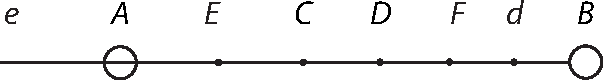
\includegraphics[width=0.54\textwidth]{%
gesamttex/edit_VIII,3/images/LH_37_05_144-145_d5_145r.pdf%
}} 
\vspace{0.5em}
\centerline{%
\lbrack\textit{Fig.~3}\rbrack%
}
% \newpage%
\vspace{1.5em}
%
\pstart
%
\edtext{}{%
\lemma{\hspace*{1,6mm}%
\lbrack\textit{Fig.~3}\rbrack%
}\killnumber%
\Cfootnote{%
Vorlage ist a.a.O., Fig.~13; Leibniz hat den Punkt \textit{F} ergänzt.%
}}%
%
%
\edlabel{37_05_144-145_22a}%
\edtext{}{% B-Footnote – "Propositio Mariotti" mit Absatz und andere B-Fn
{\xxref%
{37_05_144-145_22a}{37_05_144-145_22b}}%
\lemma{Propositio \lbrack...\rbrack\ regulam}\Cfootnote{%
\cite{00311}a.a.O., %
Prop.~XIX,
S.~115\textendash119.}}%
Propositio Mariotti\protect\index{Namensregister}{\textso{Mariotte}, Edme, Seigneur de Chazeuil ca. 1620\textendash1684} 
\edtext{\lbrack XIX.\rbrack}{%
\lemma{}%
\Bfootnote{%
IX. %
\textit{L ändert Hrsg.}%
}}
%
continet regulam\edlabel{37_05_144-145_22b} praecise eandem cum Hugeniana\protect\index{Namensregister}{\textso{Huygens} (Hugenius, Ugenius, Hugens, Huguens), Christiaan 1629\textendash1695}%
\protect\index{Sachverzeichnis}{regula Hugeniana}
%
supra decem casibus%
\protect\index{Sachverzeichnis}{decem casus Hugeniani} explicata, ideoque subjacet iisdem incommodis. Tantum demonstrationem
%
habet quae huc  
%
\edlabel{37_05_144-145_21a}%
\edtext{}{% NEUER ABSATZ UND VARIANTEN – "redit: Sint"
{\xxref%
{37_05_144-145_21a}{37_05_144-145_21b}}%
\lemma{redit:}\Bfootnote{\textit{(1)}~\textbar\ Sit \textit{streicht Hrsg.}~\textbar\ %
 $\displaystyle\frac{AC}{CB}\sqcap\displaystyle\frac{B}{A}$. Eorum \textit{(2)}~Sint \textit{AB}, \textit{(3)}~Sint~\textit{L}}}%
redit:
\pend
%
\pstart
Sint%
\edlabel{37_05_144-145_21b}
%
corpora in \textit{A}, \textit{B}, centrum gravitatis\protect\index{Sachverzeichnis}{centrum gravitatis} \textit{C}, 
%
celeritates et directiones
sint \textit{AD}, \textit{BD}. Sumatur $CE \sqcap CD$. Erunt 
%
\textit{AE},  
%
\edtext{\textit{BE} celeritates}{%
\lemma{\textit{BE}}%
\Bfootnote{%
\textit{(1)}~celeritas %
\textit{(2)}~celeritates%
~\textit{L}%
}}
%
et directiones corporum \textit{A}, \textit{B}.%
%
\edlabel{37_05_144-145_20a}%
\edtext{}{% C-Footnote – Prop XIX und Figur - überkreuzt sich mit B-Fn
{\xxref%
{37_05_144-145_20a}{37_05_144-145_20b}}%
\lemma{Hoc \lbrack...\rbrack\ versus \textit{B}}%
\Cfootnote{%
\cite{00311}a.a.O., S.~115\textendash117 %
und die dazugehörige Fig.~13.%
}}
%
Hoc Mariottus\protect\index{Namensregister}{\textso{Mariotte}, Edme, Seigneur de Chazeuil ca. 1620\textendash1684} ita demonstrat:
%
si ambo corpora essent sine Elaterio%
\protect\index{Sachverzeichnis}{elaterium} post concursum%
\protect\index{Sachverzeichnis}{concursus} simul ferrentur celeritate et directione 
aequali ipsi \textit{CD} 
%
\edtext{versus \textit{B} (\protect\vphantom)seu}{%
\lemma{versus \textit{B}}%
\Bfootnote{%
\textit{(1)}~, seu %
\textit{(2)}~(\protect\vphantom)seu%
~\textit{L}%
}}
%
celeritate et directione \textit{DF} posita \textit{F} pro \textit{C} figurae 13\protect\vphantom().
%
\edtext{Sed vis\protect\index{Sachverzeichnis}{vis}}{\lemma{Sed}\Bfootnote{\textit{(1)}~ictus idem est, \textit{(2)}~vis~\textit{L}}}
%
celeritate respectiva\protect\index{Sachverzeichnis}{celeritas respectiva} quaesita,%
\protect\index{Sachverzeichnis}{vis celeritate respectiva quaesita} seu  
%
ictus\protect\index{Sachverzeichnis}{ictus} idem est qui foret si sibi occurrissent celeritate 
%
\edtext{\textit{AC}, \textit{BC}, eo autem}{%
\lemma{\textit{AC}, \textit{BC},}%
\Bfootnote{%
\textit{(1)}~\textbar\ eo casu vero corpus \textit{A} elaterio acciperet celeritatem \textit{AC} \textit{streicht Hrsg.}~\textbar\ %
\textit{(2)}~eo autem%
~\textit{L}%
}}
casu 
%
redibit \textit{A} celeritate et directione \textit{CA}, et \textit{B} celeritate et directione \textit{CB}. Ergo \textit{A} feretur nunc celeritate et directione $CA - CD$ id est
minus \textit{EC}, quae facit \textit{AE}, sunt enim \textit{CA} et \textit{CD} directiones in contrarias partes, at \textit{B} feretur celeritate et directione $CD+CB$, id est \textit{EC}
plus \textit{CB}, seu \textit{EB} scilicet 
%
%
\edlabel{37_05_144-145_14a}%
\edtext{}{% NEUER ABSATZ UND VARIANTEN – "versus B. Elegantia"
{\xxref%
{37_05_144-145_14a}{37_05_144-145_14b}}%
\lemma{versus \textit{B}.}%
\Bfootnote{%
\textit{(1)}~Exc %
\textit{(2)}~Si duo corpora co %
\textit{(3)}~Elegantia adjicit Mariottus theoremata: %
\textit{(a)}~ut si duo %
\textit{(b)}~si %
\textit{(c)}~nempe %
\textit{L}%
}}%
versus \textit{B}.\edlabel{37_05_144-145_20b}
\pend
\newpage
%
\pstart
Elegantia adjicit Mariottus\protect\index{Namensregister}{\textso{Mariotte}, Edme, Seigneur de Chazeuil ca. 1620\textendash1684} theoremata\protect\index{Sachverzeichnis}{theorema elegans}:
%
nempe%
\edlabel{37_05_144-145_14b}
%
\edtext{\edlabel{LH_37_05_145r_prop.I.20_Mario-1}% Referenzierung für PR
prop.~20 si duo % C-Fn um einige B-Fn herum
%
\edtext{corpora elastica\protect\index{Sachverzeichnis}{corpus elasticum}}{\lemma{corpora}\Bfootnote{\textit{(1)}~aequalia \textit{(2)}~elastica~\textit{L}}}
%
quomodocunque concurrant, et post  
%
\edtext{primum concursum\protect\index{Sachverzeichnis}{concursus primus} iterum}{\lemma{primum concursum}\Bfootnote{\textit{(1)}~servatur \textit{(2)}~iterum~\textit{L}}}
%
concurrant, restituentur per secundum concursum\protect\index{Sachverzeichnis}{concursus secundus} in statum qui erat ante primum concursum\protect\index{Sachverzeichnis}{concursus primus}, quantum ad
%
propriam celeritatem, quam scilicet resument.}{\lemma{prop.~20 \lbrack...\rbrack\ resument}\Cfootnote{\cite{00311}a.a.O., Prop.~XX, S.~122\textendash124.}}
%
\edtext{Hoc ait experimento\protect\index{Sachverzeichnis}{experimentum} comprobari. % C-Fn um eine B-Fn herum
Duae inquit pilae eburneae\protect\index{Sachverzeichnis}{pila eburnea} suspendantur, quarum una triplum
%
alterius ponderet, concurrant celeritatibus aequalibus demissae ex arcu graduum duodecim. Videbimus majorem ibi quiescere, et minorem repulsam 
%
assurgere ad 24 graduum arcum. Unde si rursus decidat in majorem quiescentem, ambae aequaliter repercussae resurgent
%
\edtext{ad gradum 12\textsuperscript{mum}}{\lemma{gradum}\Bfootnote{\textit{erg.}~\textit{L}}}
%
unde primum decidere.%	%Referenzierung für PR
\edlabel{LH_37_05_145r_prop.I.20_Mario-2}}{%
\lemma{Hoc \lbrack...\rbrack\ decidere}%
\Cfootnote{%
\cite{00311}a.a.O., Prop.~XX, \textit{Preuves par experience}, S.~125f.%
}}
%
Haec propositio valde videtur rationi%
\protect\index{Sachverzeichnis}{ratio} consentanea, in pen\textlangle dula\textrangle%
\protect\index{Sachverzeichnis}{pendulum} quadam seu 
\lbrack145~v\textsuperscript{o}\rbrack\ 
%
circulari actione%
\protect\index{Sachverzeichnis}{actio circularis}, qua fieri debet, ut omnia in priorem plane statum%
\protect\index{Sachverzeichnis}{status prius} redeant.%
\edlabel{37_05_144-145_23b}%Ende der Besprechung von Mariotte
%
\pend
\count\Bfootins=1200%
\count\Afootins=1200%
\count\Cfootins=1200